\chapter{Mise en \oe uvre numérique de l'algorithme de propagation}
\label{chap:methode_numerique}

Dans ce chapitre, on propose une mise en \oe uvre numérique de l'algorithme présenté au chapitre précédent. 
\begin{enumerate}
	\item choix de la discrétisation spatiale
	\begin{itemize}
		\item représentation des carreaux de surface
		\item représentation (et calcul) des courbes d'intersection entre carreaux
	\end{itemize}
	\item intégration temporelle
	\begin{itemize}
		\item intégration explicite du champ de vitesse 
		\item construction géométrique discrète de l'EdB suivant une méthode pseudo-spectrale (exacte aux points de collocation + interpolation)
	\end{itemize}
	\item considérations sur la stabilité numérique
\end{enumerate}



%\section{Discrétisation (pseudo-)spectrale en espace}
\section{Représentation des carreaux de surface}
\subsection{État de l'art}
\begin{enumerate}
	\item harmoniques sphériques \cite{rahimian2015}
	\item polynômes trigonométriques \cite{gueyffier2015}
	\item[$\Rightarrow$] limitations géométriques (régularité globale) et topologique (périodicité)
	\item modèle \brep\ permet une plus grande flexibilité
	\item polynômes algébriques (en produit tensoriel) adaptés aux carreaux de surface
	\item CAO : Bezier, NURBS $\to$ base des polynômes de Bernstein
	\begin{itemize}
		\item $B_n^N(x) = \binom{N}{n} \left( 1 - x \right)^{N-n} x^n$ pour $0 \leq n \leq N$.
		\item positivité : pour $0 \leq x \leq 1$, $B_n^N(x) \geq 0$
		\item partition de l'unité : $\sum_{n = 0}^N B_n^N = 1$
		\item[$\to$] propriétés intéressantes pour la conception géométrique
		\begin{itemize}
			\item coefficients = points de contrôle
			\item l'enveloppe convexe des points de contrôle englobe la courbe/surface de Bézier
		\end{itemize}
		\item inconvénients :
		\begin{itemize}
			\item points de contrôle pas \emph{sur} la courbe/surface $\Rightarrow$ pas exploitables comme marqueurs lagrangiens
			\item algorithme d'évaluation (de Casteljau) numériquement stable mais coûteux $\bigO{N^2}$
		\end{itemize}
	\end{itemize}
	\item motivation le choix des polynômes de Chebyshev
\end{enumerate}

%\subsection{Polynômes de Bernstein}
%Les polynômes de Bernstein sont définis par
%\begin{equation}
%	B_n^N(x) = \binom{N}{n} \left( 1 - x \right)^{N-n} x^n,
%	\label{eq:bernstein_poly}
%\end{equation}
%pour $0 \leq n \leq N$.
%Propriétés :
%\begin{itemize}
%	\item positivité : pour $0 \leq x \leq 1$, $B_n^N(x) \geq 0$
%	\item partition de l'unité : $\sum_{n = 0}^N B_n^N = 1$
%	\item dérivée : ${B_n^N}' = N \left( B_{n-1}^{N-1} - B_n^{N-1} \right)$
%\end{itemize}
%Avantages/inconvénients
%\begin{itemize}
%	\item[$+$] coefficients = points de contrôle dans l'espace physique, sens géométrique intuitif
%	\item[$+$] partition de l'unité sur $\berninterval$ $\Rightarrow$ propriété d'enveloppe convexe
%	\item[$\pm$] algorithme d'évaluation (de Casteljau) numériquement stable mais coûteux $\bigO{N^2}$
%	\item[$-$] points de contrôle pas \emph{sur} la courbe/surface $\Rightarrow$ pas exploitables comme marqueurs lagrangiens
%	\item[$-$] peu pratiques pour réduire/élever le degré des polynômes
%\end{itemize}


\subsection{Polynômes de Chebyshev univariés}
Les polynômes de Chebyshev sont très largement utilisés dans de nombreux domaines tels que l'analyse numérique.
L'objet des sections suivantes est de rappeler la définition de cette famille de polynômes et d'en présenter brièvement les propriétés remarquables qui seront exploitées dans cette thèse. 
Nombreux sont les ouvrages consacrés aux polynômes de Chebyshev \cite{mason2002, gil2007} ainsi qu'à leur usage dans les méthodes spectrales \cite{boyd2001, canuto2006}, aussi le lecteur est invité à s'y référer pour plus de détails.

\subsubsection{Définition et principales propriétés}
\begin{definition}
	Pour $n \in \mathbb{N}$, le polynôme de Chebyshev (de première espèce) $T_n$ est défini par%un polynome de degré $n$ défini par
	\begin{equation}
		T_n(\cos \theta) = n \cos \theta.
		\label{eq:chebyshev_trigo}
	\end{equation}
\end{definition}
%De la définition \eqref{eq:chebyshev_trigo} et de l'identité trigonométrique
De cette définition et de l'identité trigonométrique $\cos n\theta + \cos (n-2)\theta = 2\cos \theta \cos (n-1)\theta$, on peut déduire la relation de récurrence suivante, pour $-1 \leq x \leq 1$, 
\begin{align}[left = \empheqlbrace\,]
	T_0(x) &= 1, \nonumber\\
	T_1(x) &= x, \nonumber\\
	T_n(x) &= 2x T_{n-1}(x) - T_{n-2}(x) \text{,\ pour\ } n \geq 2.
	\label{eq:chebyshev_recurrence}
\end{align}
Le graphe des six premiers polynômes de Chebyshev est tracé sur la \autoref{fig:chebyshev_polynomials}.\par

\begin{figure}
	\centering
	%https://tex.stackexchange.com/questions/127375/replicate-the-fourier-transform-time-frequency-domains-correspondence-illustrati
\begin{tikzpicture}[%
		ax/.style={on layer=background, black, line width=0.5pt},
		grid/.style={on layer=background, black!25, line width=0.4pt},
		tickl/.style={font=\small},
		myax/.style={}
	]%
	\begin{axis}[
	width=12cm, height=9cm,
    set layers=standard,
    %domain=-1:1,
    xmin=-1, xmax=1,
    zmin=-1, zmax=1,
    samples y=1,
    view={40}{30},
    %hide axis,
    axis line style={draw=none},
    tick style={draw=none},
    grid = none,
    axis lines* = left,
    unit vector ratio*=4 3 1,
    %xtick=\empty, ytick=\empty, ztick=\empty,
    xtick={-1,-0.5,0,0.5,1},
    ytick={0,1,2,3,4,5},
    ztick={-1,0,1},
    %xlabel={$x$},
    %ylabel={$n$},
    %zlabel={$T_n(x)$},
    yticklabels=\empty,
    %zticklabels=\empty,
    no marks,
    samples=201,
    every tick label/.append style={font=\small},
    %tick align=outside,
%    cycle list/GnBu-9,%RdYlBu-6,%Spectral-6,
%	cycle multiindex* list={GnBu-9},%RdYlBu-6}%Spectral-6}
    clip=false
]
% x,z grid lines (at y=cst)
\foreach \y in {0,1,...,5}{%
	\foreach \x in {{-0.5},{0},{0.5},{1}}{
		\begingroup\edef\temp{\endgroup\noexpand\draw [grid] (axis cs:\x,\y,-1) -- ++ (axis direction cs:0,0,2);}\temp
	}
	\foreach \z in {{0},{1}}{
		\begingroup\edef\temp{\endgroup\noexpand\draw [grid] (axis cs:-1,\y,\z) -- ++ (axis direction cs:2,0,0,0);}\temp
	}
}
\pgfplotsinvokeforeach{0,1,...,5}{%
	\addplot3+[domain=-1:1]	({x},#1,{ cos(#1*acos(x)) });
%	\node[font=\footnotesize, anchor=west, inner sep=0] 
%		at (axis cs:1,#1,-0.3) {$n = #1$};
	\draw [ax] (axis cs:-1,#1,-1) -- ++ (axis direction cs:2,0,0); % x-axis
	\draw [ax] (axis cs:-1,#1,-1) -- ++ (axis direction cs:0,0,2); % z-axis
}%
% x,z ticks
\foreach \y in {0,1,...,5}{%
	\foreach \x in {{-1},{-0.5},{0},{0.5},{1}}{
		\begingroup\edef\temp{\endgroup\noexpand\draw [ax] (axis cs:\x,\y,-1) -- ++ (axis direction cs:0,0,0.2);}\temp
	}
	\foreach \z in {{-1},{0},{1}}{
		\begingroup\edef\temp{\endgroup\noexpand\draw [ax] (axis cs:-1,\y,\z) -- ++ (axis direction cs:0.05,0,0,0);}\temp
	}
}
% x, z tick labels and grid lines
%\pgfplotsinvokeforeach{-1,-0.5,0,0.5,1}{
%	\node[anchor=north, myax, tickl, xshift=-4pt] at (axis cs:#1,0,-1.1) {$#1$};
%%	\draw [grid] (axis cs:#1,0,-1) -- ++ (axis direction cs:0,5,0);
%}
%\pgfplotsinvokeforeach{-1,0,1}{
%	\node[anchor=east, myax, tickl] at (axis cs:-1,0,#1) {$#1$};
%%	\draw [grid] (axis cs:-1,0,#1) -- ++ (axis direction cs:0,5,0);
%}
% x,z labels
\node[anchor=north west, myax] at (axis cs:0,-1.1,-1) {$x$};
\node[anchor=south, rotate=90, myax, inner sep=7mm] at (axis cs:-1,0,0) {$T_n(x)$};
%
% y axis
\draw[ax, -latex] (axis cs:1.25,0,-1) -- ++ (axis direction cs:0,5.5,0) node[anchor=south west] {$n$};
\pgfplotsinvokeforeach{0,1,...,5}{%
	\draw[ax] (axis cs:1.25,#1,-1) -- ++ (axis direction cs:-0.05,0,0);
	\node[anchor=north west, myax, tickl] at (axis cs:1.25,#1,-1) {$#1$};
}
%\foreach \n in {0,1,...,5}{%
%	\node[font=\footnotesize, anchor=west, inner sep=0] 
%		at (axis cs:1,\n,-0.3) {$n = \n$};
%	\draw [ax] (axis cs:-1,\n,-1) -- ++ (axis direction cs:2,0,0); % x-axis
%	\draw [ax] (axis cs:-1,\n,-1) -- ++ (axis direction cs:0,0,2); % z-axis
%	\foreach \z in {-1,0,1}{%
%		\draw [ax] (axis cs:-1,\n,\z) -- ++ (axis direction cs:0.025,0,0);
%	}%
%	\foreach \x in {-1,-0.5,0,0.5,1}{%
%		\draw [ax] (axis cs:\x,\n,-1) -- ++ (axis direction cs:0,0,0.1);
%	}%
%}%
\end{axis}
\end{tikzpicture}
	\caption{Graphe des six premiers polynômes de Chebyshev.}% $(n=0,\ldots,5)$ sur l'intervalle $\chebinterval$.}
	\label{fig:chebyshev_polynomials}
\end{figure}

$T_n$ est un polynôme de degré $n$ %de coefficient dominant $2^{n-1}$ 
qui atteint ses extrema locaux sur $\chebinterval$ aux $n+1$ n\oe uds de Chebyshev-Gauss-Lobatto (CGL)%\footnote{Seuls les $n-1$ n\oe uds intérieurs sont réellement des extrema au sens où la dérivée s'y annule. A noter également que ces n\oe uds sont rangés en ordre décroissant.}
\begin{equation}
	x_k = \cos \frac{k \pi}{n},
	\label{eq:cgl_nodes}
\end{equation}
pour $0 \leq k \leq n$. 
Seuls les $n-1$ n\oe uds intérieurs sont réellement des extrema au sens où la dérivée s'y annule. 
À noter également que ces n\oe uds sont rangés en ordre décroissant.\par

\begin{figure}
	\centering
	\begin{tikzpicture} 
	\begin{axis}[%
		width=8cm, height=6cm,
		axis lines*=left,
		xmin=-1.0, xmax=1.0, ymin=-1.0, ymax=1.0,
		grid=major,
		clip marker paths=false,
		enlargelimits={abs=0.05},
		]%
		\addplot+[samples=200, domain=0:pi, no marks, mycolor_6] ({cos(deg(x))}, {cos(5*deg(x))});%
		% extrema
		\addplot+[samples=6, domain=0:pi, ycomb, dashed, mark=none, black] ({cos(deg(x))}, {cos(5*deg(x))});%
		\addplot+[samples=6, domain=0:pi, only marks, mark=*, black] ({cos(deg(x))}, {0});%
		% zeros
%		\pgfplotsinvokeforeach{0,...,4}{
%			\addplot+[mark=*, red] coordinates {(cos((2.0*#1+1.0)*180.0/10.0),0)};
%		}
	\end{axis} 
\end{tikzpicture}
%	\caption{N\oe uds de Chebyshev-Gauss-Lobatto pour $n = 6$ (extrema locaux du polynome $T_6$ sur l'intervalle $\chebinterval$).}
	\caption{N\oe uds de Chebyshev-Gauss-Lobatto (extrema locaux) du polynôme $T_5$.}% sur l'intervalle $\chebinterval$.}
	\label{fig:cgl_nodes}
\end{figure}

Comme illustré sur la \autoref{fig:cgl_nodes}, ces extrema sont alternativement des maxima puis des minima, tous égaux en valeur absolue
\begin{equation}
	T_n(x_k) = (-1)^{k}.
	\label{eq:chebyshev_equioscillation}
\end{equation}

Cette propriété d'\emph{équioscillation} a pour conséquence le théorème suivant.
\begin{theoreme}
	Le polynôme %$p_{N-1}$ 
	de degré $N-1$ qui donne la meilleure approximation uniforme (\ie en norme $L_\infty$) %de la fonction $x \mapsto x^N$ est $p_{N-1} : x \mapsto x^N - 2^{1 - N} T_n(x)$. 
du polynôme %$q : x \mapsto \sum_{n=0}^{N} a_n x^n$
$q = \sum_{n=0}^{N} a_n X^n$ 
sur l'intervalle $\chebinterval$ est
	\begin{equation}
		p_{N-1} = q - 2^{1-N} a_N T_N,
	\end{equation}
	et, pour tout $x \in \chebinterval$,
	%La meilleure approximation %uniforme (\ie en norme $L_\infty$) 
	%polynomiale de degré $N - 1$ en norme $L_\infty$ de la fonction $x \mapsto x^N$ sur $\chebinterval$ est la fonction $p_N : x \mapsto x^N - 2^{1 - N} T_n(x)$ et
	\begin{equation}
		%\norminf{q - p_{N-1}} = 2^{1-N} \left| a_N \right|.
		\left| q(x)-  p_{N-1}(x)\right| \leq 2^{1-N} \left| a_N \right|,
	\end{equation}
	l'égalité étant atteinte aux $N+1$ n\oe uds CGL de $T_N$.
\end{theoreme}
Ce théorème trouve une application immédiate dans l'économisation des séries \textit{(à développer\ldots)}.


\subsubsection{Approximation de fonctions}
%somme partielle, polynôme d'interpolation, erreurs de troncature et d'aliasing, DCT/FCT
Notons $\Ltwospace$ l'espace de Hilbert des fonctions de carré intégrable sur $\chebinterval$, muni du produit scalaire
\begin{equation}
	\scalprod{f}{g} =
	\int_{-1}^{1} \frac{f(x) g(x)}{\sqrt{1 - x^2}} \dx{x} .
	\label{eq:chebyshev_scalar_product}
\end{equation}

La famille des polynômes de Chebyshev est une base orthogonale et maximale de cet espace, et pour tous $m,n \in \mathbb{N}$,
\begin{equation}
	\scalprod{T_m}{T_n} =
	\frac{\pi}{2} \alpha_n \delta_{m,n},
	\label{eq:chebyshev_orthogonality}
\end{equation}
où $\delta_{\cdot,\cdot}$ représente le symbole de Kronecker, et
\begin{equation}
	\alpha_n = 
	1 + \delta_{0,n}.
%	\begin{cases}
%	 2 & \text{\ si\ } n = 0,   \\ 
%	 1 & \text{\ si\ } n > 0.\\ 
%	\end{cases}
\end{equation}

Toute fonction $f \in \Ltwospace$ peut alors être représentée par sa série de Chebyshev
\begin{equation}
	f = \sum_{n=0}^{\infty} \hat{f}_n T_n,
	\label{eq:chebyshev_series}
\end{equation}
dont les coefficients $\hat{f}_n$ sont obtenus en prenant le produit scalaire
\begin{align}
	\hat{f}_n 
	&= \frac{\scalprod{f}{T_n}}{\scalprod{T_n}{T_n}}, \nonumber \\
	&= \frac{2}{\pi \alpha_n} \int_{-1}^{1} \frac{f(x) T_n(x)}{\sqrt{1 - x^2}} \dx{x} .
	\label{eq:chebyshev_series_coeffs}
\end{align}

La somme partielle
\begin{equation}
	\truncseries{f}{N} = \sum_{n=0}^{N} \hat{f}_n T_n
	\label{chebyshev_truncated_series}
\end{equation}
est le projeté orthogonal de $f$ sur le sous-espace $\polyspace{N}$ de $\Ltwospace$ des polynômes de degré au plus $N$.
Il s'agit donc de l'élément de $\polyspace{N}$ le plus proche de $f$, au sens de la norme induite par le produit scalaire \eqref{eq:chebyshev_scalar_product}.\par
La somme partielle $\truncseries{f}{N}$ est également proche de la meilleure approximation uniforme de $f$ par un polynôme de degré N. 
En effet, si $f$ est continue sur $\chebinterval$, alors
\begin{equation}
	\norminf{f - \truncseries{f}{N}} 
	\leq 
	\left(1 + \lambda_N \right) 
	\min_{p \in \polyspace{N}} \norminf{f - p},
	\label{eq:chebyshev_near_minimax}
\end{equation}
où la constante de Lebesgue $\lambda_N = 1.27\ldots + \frac{4}{\pi^2} \log N + \bigO{N^{-1}}$ croît lentement avec $N$ ($\lambda_{500} \approx 3.8$).\par

Dans le contexte particulier de la résolution numérique d'équations aux dérivées partielles, %les séries de Chebyshev représentent un puissant outil pour l'approximation de fonctions possédant des dérivées continues, pour lesquelles la somme partielle $\truncseries{f}{N}$ converge très rapidement.
on s'intéresse à l'approximation de fonctions qui possèdent des dérivées continues.
Pour de telles fonctions, les séries de Chebyshev convergent très rapidement. 
En effet, à l'aide d'une intégration par parties répétée, on peut montrer que la relation \eqref{eq:chebyshev_series_coeffs} implique le théorème suivant.
\begin{theoreme}
	Si $f$ est $p-1$ fois dérivable presque partout sur \chebopeninterval\ et si $f^{(p-1)}$ est de variation bornée sur \chebinterval, alors 
	\begin{equation}
		\hat{f}_n = \bigO{n^{-p}}.
		\label{eq:chebyshev_convergence_coef_algebraic}
	\end{equation}
	En particulier, si $f \in \contdiff{\infty}\chebinterval$ alors la suite des coefficients $\hat{f}_n$ décroît plus rapidement que n'importe quelle puissance négative de $n$.\par
	En outre, si $f$ admet une extension analytique dans une région %\footnote{Il s'agit de la région bornée délimitée par l'ellipse de foyers $\pm 1$ et dont la somme des demi-axes vaut $r$.} 
	du plan complexe contenant le segment \chebinterval , alors il existe $r > 1$ tel que
	\begin{equation}
		\hat{f}_n = \bigO{r^{-n}}.
		\label{eq:chebyshev_convergence_coef_geometric}
	\end{equation}
\end{theoreme}
\par

Puisque $\left|T_n \right| \leq 1$ sur \chebinterval\ pour tout entier $n$, il s'ensuit que l'\textit{erreur de troncature} est bornée par la somme des valeurs absolues des coefficients négligés
\begin{equation}
	\norminf{f - \truncseries{f}{N}} \leq \sum_{n=N+1}^{\infty} 
	\left| \hat{f}_n \right|.
	\label{eq:chebyshev_truncation_error_bound}
\end{equation}

Or, si les coefficients $\hat{f}_n$ convergent avec une rapidité algébrique de la forme \eqref{eq:chebyshev_convergence_coef_algebraic}, alors\par
\begin{equation}
	\norminf{f - \truncseries{f}{N}} 
	= \bigO{N^{1-p}} 
	= \bigO{N \left| \hat{f}_N \right|}.
	\label{eq:chebyshev_truncation_error_estimator_algebraic}
\end{equation}

Si, en revanche, la convergence est géométrique (\ie de la forme \eqref{eq:chebyshev_convergence_coef_geometric}), alors 
\begin{equation}
	\norminf{f - \truncseries{f}{N}} 
	= \bigO{r^{-N}}
	= \bigO{\left| \hat{f}_N \right|}.
	\label{eq:chebyshev_truncation_error_estimator_geometric}
\end{equation}

Les règles empiriques \eqref{eq:chebyshev_truncation_error_estimator_algebraic} et \eqref{eq:chebyshev_truncation_error_estimator_geometric} permettent d'estimer efficacement l'erreur de troncature qui, en pratique, est inconnue. \textit{(dévélopper\ldots)}

\par\bigskip
\textit{Motivation pour interpolation\ldots}

%En pratique, l'intégrale \eqref{eq:chebyshev_series_coeffs} ne peut pas être calculée analytiquement  \ldots\\
Les polynômes de Chebyshev satisfont une seconde relation d'orthogonalité, dite \guillemets{discrète}, pour $0 \leq n \leq N$ et $m \geq n$,
\begin{equation}
	%\sum_{k=0}^{N}{''} T_m(x_k) T_n(x_k) = 
	\sum_{k=0}^{N} \frac{1}{\beta_k} T_m(x_k) T_n(x_k) = 
	\frac{N}{2} \beta_n \delta_{m,\pm n \bmod{2N}},
	\label{eq:chebyshev_discrete_orthogonality}
\end{equation}
où $\family{x}{k}{0}{N}$ sont les n\oe uds CGL de $T_N$ définis par l'équation \eqref{eq:cgl_nodes} et
\begin{equation}
	\beta_n = 
	1 + \delta_{0,n} + \delta_{N,n}.
%	\begin{cases}
%	 2 & \text{\ si\ } n = 0 \text{\ ou\ } N,   \\ 
%	 1 & \text{\ si\ } 0 < n < N.\\ 
%	\end{cases}
\end{equation}

%Le double prime dans l'équation \eqref{eq:chebyshev_discrete_orthogonality} signifie que les premier et dernier termes de la somme sont divisés par 2.
\par


Soit $\interpolant{f}{N}$ l'unique polynôme de $\polyspace{N}$ qui interpole $f$ aux $N+1$ n\oe uds CGL de $T_N$
\begin{equation}
	\interpolant{f}{N}(x_k) = f(x_k).
	\label{eq:chebyshev_interpolation_cgl}
\end{equation}

Ce polynôme peut s'exprimer dans la base de Chebyshev
\begin{equation}
	\interpolant{f}{N} = \sum_{n=0}^{N} \tilde{f}_n T_n.
	\label{eq:chebyshev_interpolant}
\end{equation}

En utilisant les relations \eqref{eq:chebyshev_interpolant}, \eqref{eq:chebyshev_interpolation_cgl} et \eqref{eq:chebyshev_discrete_orthogonality}, on peut alors déduire les coefficients $\tilde{f}_n$ à partir des valeurs de $f$ en ces n\oe uds
\begin{equation}
	%\tilde{f}_n = \frac{2}{\beta_n N} \sum_{k=0}^{N} {''} f(x_k) \cos \frac{n k \pi}{N}.
	\tilde{f}_n = \frac{2}{\beta_n N} \sum_{k=0}^{N} \frac{1}{\beta_k} f(x_k) \cos \frac{n k \pi}{N}.
	\label{eq:chebyshev_dct}
\end{equation}

L'équation \eqref{eq:chebyshev_dct} définit ainsi une transformation discrète [de l'espace \guillemets{physique} vers l'espace \guillemets{spectral}]\footnote{reformuler!}. 
Par ailleurs, des relations \eqref{eq:chebyshev_interpolation_cgl}, \eqref{eq:chebyshev_interpolant} et \eqref{eq:chebyshev_trigo}, on peut déduire la transformation inverse
\begin{equation}
	f(x_k) = \sum_{n=0}^{N} \tilde{f}_n \cos \frac{n k \pi}{N}.
	\label{eq:chebyshev_idct}
\end{equation}

Les équations \eqref{eq:chebyshev_dct} et \eqref{eq:chebyshev_idct} décrivent des transformations en cosinus discrètes (DCT), qui peuvent être effectuées efficacement à l'aide d'un algorithme de transformation de Fourier rapide (FFT) pour un coût asymptotique de $\bigO{N \log N}$ opérations.
\par
Les coefficients $\tilde{f}_n$ peuvent être reliés aux coefficients $\hat{f}_n$ par la relation
\begin{equation}
	\tilde{f}_n = \hat{f}_n + 
	\begin{cases}
		\displaystyle\sum_{j=1}^{\infty} \hat{f}_{2jN + n} & \text{\ si\ } n = 0 \text{\ ou\ } N,   \\[4ex]
		\displaystyle\sum_{j=1}^{\infty} \left( \hat{f}_{2jN - n} + \hat{f}_{2jN + n} \right) & \text{\ si\ } 0 < n < N. 
	\end{cases}
	\label{eq:chebyshev_aliasing}
\end{equation}

Cette relation met en évidence le phénomène d'\anglais{aliasing}, qui traduit le fait que les polynômes $T_n$ et $T_{\pm n \bmod{2N}}$ prennent les mêmes valeurs aux n\oe uds $\family{x}{k}{0}{N}$, comme illustré sur la \autoref{fig:aliasing_cgl}.
La différence entre le polynôme d'interpolation $\interpolant{f}{N}$ et la somme partielle $\truncseries{f}{N}$ est l'\textit{erreur d'aliasing}, qui est orthogonale à l'erreur de troncature\footnote{$\normtwo{\cdot}$ désigne ici la norme induite par le produit scalaire \eqref{eq:chebyshev_scalar_product}.}
\begin{equation}
	\normtwo{f - \interpolant{f}{N}}^2 = 
	\normtwo{f - \truncseries{f}{N}}^2 + 
	\normtwo{\interpolant{f}{N} - \truncseries{f}{N}}^2.
	\label{eq:chebyshev_aliasing_esrror}
\end{equation}

L'erreur d'approximation due à l'interpolation est donc toujours supérieure à l'erreur liée à la troncature de la série de Chebyshev.
Si $f$ est régulière, la suite des coefficients $\hat{f}_n$ converge rapidement vers zéro, si bien que l'erreur d'aliasing reste faible, à condition que le degré de troncature $N$ soit choisi suffisamment grand.
En outre, de la relation \eqref{eq:chebyshev_aliasing} on déduit que pour tout $x \in \chebinterval$,
\begin{equation}
	\left| f(x) - \interpolant{f}{N}(x) \right| \leq 2 \sum_{n>N} \left| \hat{f}_n \right|.
\end{equation}
L'erreur d'approximation due à l'interpolation est donc \textit{au pire} supérieure à l'erreur de troncature par un facteur 2.
L'erreur d'aliasing peut cependant devenir problématique lorsqu'elle est amplifiée par les non-linéarités présentes dans les équations que l'on sera amené à résoudre. 
Nous reviendrons sur ce point dans la \autoref{section:instabilités} lorsque nous aborderons \ldots

\begin{figure}
	\centering
	\begin{tikzpicture}
		\begin{axis}[%
			width=8cm, height=6cm,
			axis lines*=left,
			xmin=-1.0, xmax=1.0, ymin=-1.0, ymax=1.0,
			grid=major,
%			xtick = {-1,0,1},
%			ytick = {-1,0,1},
			clip marker paths=false,
			enlargelimits={abs=0.05},
			]%
			\addplot+[samples=200, domain=0:pi, no marks] ({cos(deg(x))}, {cos(3*deg(x))});% T_3
			\addplot+[samples=200, domain=0:pi, no marks] ({cos(deg(x))}, {cos(7*deg(x))});% T_7
			\addplot+[samples=500, domain=0:pi, no marks] ({cos(deg(x))}, {cos(13*deg(x))});% T_13
%			\addplot+[domain=-1:1, no marks, samples=200, black, dotted] {16*x^5 - 20*x^3 + 5*x};% T_5
			\addplot+[samples=6, domain=0:pi, ycomb, dashed, mark=*, black] ({cos(deg(x))}, {cos(3*deg(x))});% noeuds CGL de T_5
		\end{axis}
	\end{tikzpicture}
	\caption{Les polynômes $T_n (\protect\legenddash{mycolor_1})$, $T_{2N - n} (\protect\legenddash{mycolor_2})$ et $T_{2N + n} (\protect\legenddash{mycolor_3})$ sont indiscernables aux n\oe uds CGL de $T_N$ (ici, $n = 3$ et $N = 5$).}
	\label{fig:aliasing_cgl}
\end{figure}


\subsubsection{Évaluation d'une somme partielle}
Par la suite, nous serons amenés à évaluer à maintes reprises des sommes de la forme
\begin{equation}
	s_N = \sum_{n=0}^N \hat{s}_n T_n
	\label{eq:chebyshev_sum}
\end{equation}
en des points autres que les n\oe uds CGL.
Plutôt que de réécrire cette somme dans la base canonique de $\polyspace{N}$, il est intéressant de tirer parti de la relation \eqref{eq:chebyshev_recurrence}. 
En introduisant la suite récurrente
\begin{equation}
	b_n(x) = 
	\begin{cases}
	 0 & \text{\ si\ } n > N,   \\ 
	 \hat{s}_n - b_{n+2}(x) + 2x b_{n+1}(x) & \text{\ si\ } 0 \leq n \leq N,
	\end{cases}
\end{equation}
on obtient, pour $-1 \leq x \leq 1$,%
\def\px{}%{(x)}%
\begin{align*}
	s_N\px 
	&= \hat{s}_0 T_0\px + \hat{s}_1 T_1\px + \ldots + \hat{s}_{N-2} T_{N-2}\px + \hat{s}_{N-1} T_{N-1}\px + \hat{s}_N T_N\px, \\
	&= \hat{s}_0 T_0 \px
	+ \hat{s}_1 T_1 \px
	+ \ldots 
	+ \left(\hat{s}_{N-2} - b_{N}\px\right) T_{N-2} \px
	+ \left(\hat{s}_{N-1} - b_{N+1}\px + 2x b_{N}\px \right) T_{N-1}\px, \\
	&= \hat{s}_0 T_0 \px
	+ \hat{s}_1 T_1 \px
	+ \ldots 
	+ \left(\hat{s}_{N-3} - b_{N-1}\px\right) T_{N-3} \px
	+ b_{N-2}\px T_{N-2}\px, \\
	& \ldots\\
	&= \left( \hat{s}_0 - b_2\px \right) T_0\px + b_1\px T_1\px, \\
	&= \hat{s}_0 - b_2\px + b_1\px x,
\end{align*}
et enfin
\begin{equation}
	s_N(x) = b_0(x) - x b_1(x).
\end{equation}

L'exécution de cet algorithme de sommation --- proposé par Clenshaw \cite{clenshaw1955} --- requiert seulement $\bigO{N}$ opérations. %, ce qui le rend plus efficace que l'algorithme de Casteljau (dont la complexité est asymptotiquement quadratique). 
La sommation de Clenshaw est donc un moyen efficace et numériquement stable pour évaluer des séries de Chebyshev.

\subsubsection{Dérivation}
%% Dérivation
(versions matricielle (espace physique) et récursive (espace spectral)\par
quadrature de Clenshaw-Curtis)\par

En posant $x = \cos\theta$, il vient, d'après \eqref{eq:chebyshev_trigo},
\begin{equation}
	T_n'(x) := \dfdx{T_n(x)}{x} = \frac{n \sin n\theta}{\sin \theta}.
\end{equation}

Ainsi, de l'identité $2 \cos n \theta \sin \theta = \sin(n+1)\theta - \sin(n-1)\theta$, on peut déduire la relation 
\begin{equation}
	2 T_n = \frac{T'_{n+1}}{n+1} - \frac{T'_{n-1}}{n-1} ,
	\label{eq:chebyshev_relation_deriv_3termes}
\end{equation}
pour $n \geq 2$.
\\
Soit $f \in \contdiff{k}\chebinterval$.
On approche la dérivée $k$-ième $\deriv{f}{k}$ de $f$ par la dérivée $k$-ième du polynôme d'interpolation $\interpolant{f}{N}$
\begin{equation}
	\interpderiv{f}{N}{k} := \deriv{ \left( \interpolant{f}{N} \right) }{k}.
	\label{eq:chebyshev_def_interpderiv}
\end{equation}
En général, les opérations de dérivation et d'interpolation ne commutent pas, \ie
\begin{equation}
	\interpderiv{f}{N}{k} \neq \interpolant{ \left( \deriv{f}{k} \right) }{N}.
\end{equation}

Les valeurs aux n\oe uds CGL de cette dérivée peuvent être exprimées comme une combinaison linéaire des valeurs de $f$ en ces mêmes n\oe uds
\begin{equation}
	\colvec{ 
		\interpderiv{f}{N}{k}(x_0) \\ 
		\vdots \\
		\interpderiv{f}{N}{k}(x_N)
		}
	=
	{\left( \mathbf{D}_N \right)}^k
	\colvec{ 
		f(x_0) \\ 
		\vdots \\
		f(x_N)
		},
	\label{eq:chebyshev_diff_at_cgl}
\end{equation}
où $\mathbf{D}_N$ est la matrice de différentiation \cite{canuto2006}
\def\cvsp{2.5ex}
\begin{equation}
	\left( \mathbf{D}_N \right)_{i,j} =
	\begin{cases}
	 \dfrac{2N^2 + 1}{6} & \text{\ si\ } i = j = 0,   \\[\cvsp]
	 -\dfrac{2N^2 + 1}{6} & \text{\ si\ } i = j = N,   \\[\cvsp]
	 -\dfrac{x_i}{2 \sin^2 \frac{i \pi}{N}} & \text{\ si\ } 0 < i = j < N, \\[\cvsp]
	 -\dfrac{(-1)^{i+j} \beta_i}{2 \beta_j \sin\frac{(i+j)\pi}{2N} \sin\frac{(i-j)\pi}{2N}} & \text{\ si\ } i \neq j.
	\end{cases}
	\label{eq:chebyshev_diff_matrix}
\end{equation}

Alternativement, il est intéressant de construire explicitement le polynôme dérivé $\interpderiv{f}{N}{k}$ comme une somme de la forme 
\begin{equation}
	\interpderiv{f}{N}{k} = \sum_{n=0}^{N-k} \deriv{\tilde{f}}{k}_n T_n.
\end{equation} 
\textit{Développer motivation\ldots}

\par
La relation \eqref{eq:chebyshev_relation_deriv_3termes} implique que, pour tout $n \in \mathbb{N}$,
\begin{equation}
	2 (n + 1) \tilde{f}_{n+1} = \alpha_n \deriv{\tilde{f}}{1}_n - \deriv{\tilde{f}}{1}_{n+2}.
	\label{eq:chebyshev_prim_recurrence}
\end{equation}
Les coefficients $\deriv{\tilde{f}}{1}_n$ peuvent ainsi être calculés suivant la relation de récurrence
\begin{equation}
	\deriv{\tilde{f}}{1}_n = 
	\frac{1}{\alpha_n} \left( 2 (n + 1) \tilde{f}_{n+1} + \deriv{\tilde{f}}{1}_{n+2} \right).
	\label{eq:chebyshev_diff_recurrence}
\end{equation}
Plus généralement, les coefficients de Chebyshev de la dérivée $k$-ième vérifient
\begin{equation}
	\deriv{\tilde{f}}{k}_n = 
	\frac{1}{\alpha_n} \left( 2 (n + 1) \deriv{\tilde{f}}{k-1}_{n+1} + \deriv{\tilde{f}}{k}_{n+2} \right).
	\label{eq:chebyshev_diffp_recurrence}
\end{equation}

Cette méthode + FFT permet d'évaluer les dérivées aux n\oe uds CGL pour $\bigO{N + N \log N} = \bigO{N \log N}$, qui est asymptotiquement (au-delà de $N \approx 16$) plus efficace que le produit matrice-vecteur \eqref{eq:chebyshev_diff_at_cgl} ($\bigO{N^2}$).
\par
Toutefois, comme l'ont fait remarquer Wengle et Seinfeld \cite{wengle1978}, l'algorithme récursif \eqref{eq:chebyshev_diffp_recurrence} peut amplifier les erreurs d'arrondi commises sur les plus petits coefficients $\deriv{\hat{f}}{k-1}_{n}$ et ainsi compromettre la précision de \emph{tous} les coefficients $\deriv{\hat{f}}{k}_{n}$. 
Un moyen simple de remédier à ce problème consiste à mettre à zéro les coefficients $\deriv{\hat{f}}{k-1}_{n}$ inférieurs en valeur absolue à un seuil donné, choisi en fonction de la précision machine $\epsilon_M$. 
(Un seuil égal à $10 \epsilon_M$ semble être un bon choix \textit{(détailler\ldots)}.)

\par\bigskip

[Illustration de la qualité de l'approximation d'une fonction analytique (et ses dérivées)par le polynôme d'interpolation (et ses dérivées) (voir \autoref{fig:spectral_convergence_function} et \autoref{fig:spectral_convergence})]

\begin{figure}%[!htp]
\centering%
\begin{tikzpicture}%
\begin{axis}[%
	width=8cm, height=6cm,
	axis lines*=left,
	xmin=-1.0, xmax=1.0,
	ymin=-1.0, ymax=1.0,
	grid=major,
	ylabel={\small $\deriv{f}{k} \norminf{\deriv{f}{k}}^{-1}$},
%	xtick = {-1,0,1},
%	ytick = {-1,0,1},
	clip marker paths=false,
	%enlargelimits={abs=0.05},
	]%
	\pgfplotsinvokeforeach{1,...,3}{
		\addplot+[no marks] table[x index=0, y index=#1] {figures/data/Chebyshev/x_f0_f1_f2.dat};%
		%\addplot+[no marks] (x, {cos(3*x + #1)});
	}
\end{axis}%
\end{tikzpicture}%
\caption{Graphes de la fonction $f : x \mapsto e^{\sin 3 x^3}$ et ses dérivées $\deriv{f}{k}$ ($k = 0 (\protect\legenddash{mycolor_1}), \; 1 (\protect\legenddash{mycolor_2}), \; 2 (\protect\legenddash{mycolor_3})$).}%
\label{fig:spectral_convergence_function}%
\end{figure}

\begin{figure}%[!htp]
\centering%
\hspace*{\fill}%
\subbottom[Erreur d'approximation par le polynôme $\interpderiv{f}{N}{k}$.]{%
\begin{tikzpicture}%
\begin{semilogyaxis}[
	width=6.7cm, height=6cm,
	xmin=0, xmax=100,
	ymin=1.0e-16, ymax=1.0e2,
	grid=both,
	axis x line*=bottom,
	axis y line*=left,
	xlabel={$N\vphantom{n}$},
	ylabel={\small $\norminf{\interpderiv{f}{N}{k} - \deriv{f}{k}} \norminf{\deriv{f}{k}}^{-1}$},
	xtick distance=25,
	legend pos=north east,
	legend style={font=\small},
	cycle list shift=-1
	]%
	%\addplot+[dashed, color=black, no marks, very thick][domain=40:60] {0.5*exp(-0.57*x)} node[pos=0.5, anchor=north east, font=\footnotesize, inner sep=1pt] {$1.8^{-N}$};%
	\addplot+[dashed, color=black, no marks, very thick][domain=40:60] {0.5*exp(-0.57*x)};%
	\addlegendentry{$1.8^{-N}$}
	\pgfplotsinvokeforeach{1,...,3}{
		\addplot+ table[x index=0, y index=#1] {figures/data/Chebyshev/convergence_DNkf.dat};%
	}
\end{semilogyaxis}%
\end{tikzpicture}%
\label{subfig:spectral_convergence_Linf}%
}%
\hspace{4mm}%
%\hfill%
\subbottom[Spectre des coefficients de Chebyshev.]{% du polynôme $\interpderiv{f}{80}{k}$.]{%
\begin{tikzpicture}%
\begin{semilogyaxis}[%
	width=6.7cm, height=6cm,
	xmin=0, xmax=100,
	ymin=1.0e-16, ymax=1.0e2,
	grid=major,
	axis y line*=right,
	axis x line*=bottom,
	xlabel={$n\vphantom{N}$},
	ylabel={},
	ylabelv right={$\left | \tilde{f}_n^{(k)} \right |$},
	ylabel near ticks, 
	yticklabel pos=right,
	yticklabels={\empty},
	xtick distance=25,
	legend pos=north east,
	legend style={font=\small},
	cycle list shift=-1
	]%
%	\addplot+[dashed, color=black, no marks, very thick][domain=40:60] {0.5*exp(-0.57*x)} node[pos=0.5, anchor=north east, font=\footnotesize, inner sep=1pt] {$1.8^{-n}$};
	\addplot+[dashed, color=black, no marks, very thick][domain=40:60] {0.5*exp(-0.57*x)};
	\addlegendentry{$1.8^{-n}$}
	\pgfplotsinvokeforeach{0,...,2}{
		\addplot+[only marks] table[x expr=\coordindex, y index=#1] {figures/data/Chebyshev/coef_DNkf.dat};%
	}
\end{semilogyaxis}%
\end{tikzpicture}%
\label{subfig:spectral_convergence_coef}%
}
\hspace*{\fill}%
\caption{Décroissance exponentielle de l'erreur d'approximation et des coefficients de Chebyshev pour la fonction analytique $f : x \mapsto e^{\sin 3 x^3}$ et ses dérivées $\deriv{f}{k}$ ($k = 0 (\protect\legendsquare{mycolor_1}), 1 (\protect\legenddot{mycolor_2}), 2 (\protect\legendtriangle{mycolor_3})$).}%
\label{fig:spectral_convergence}%
\end{figure}


\subsubsection{Intégration}
\label{section:clenshaw_curtis_quadrature}
La primitive de $\interpolant{f}{N}$ qui s'annule en $-1$
\begin{equation}
	\interpprim{f}{N} := x \mapsto \int_{-1}^{x} \interpolant{f}{N}(t) \dx{t}
\end{equation}

est un polynôme de degré $N+1$
\begin{equation}
	\interpprim{f}{N} = \sum_{n=0}^{N+1} \prim{\tilde{f}}{1}_n T_n.
\end{equation}

\eqref{eq:chebyshev_prim_recurrence} implique 
\begin{equation}
	\prim{\tilde{f}}{1}_n = \frac{\alpha_n \tilde{f}_{n-1} - \tilde{f}_{n+1}}{2n},
\end{equation}
pour $n \geq 1$ et, puisque $\interpprim{f}{N}(-1) = 0$, on a
\begin{equation}
	\prim{\tilde{f}}{1}_0 = - \sum_{n=1}^{N+1} (-1)^n \prim{\tilde{f}}{1}_n.
\end{equation}

\begin{equation}
	\int_{-1}^{x} f(t) \dx{t} 
	\approx \interpprim{f}{N}(x).
\end{equation}
En particulier,
\begin{equation}
	\int_{-1}^{1} f(t) \dx{t} 
	\approx 
	\interpprim{f}{N}(1)
	=
	\sum_{\mathclap{\substack{n = 0\\n \text{ pair}}}}^{N} \frac{2 \tilde{f}_n}{1 - n^2},
\end{equation}
et
\begin{equation}
	\left| \int_{-1}^{1} f(x) \dx{x} - \interpprim{f}{N}(1) \right|
	\approx
	\left|\frac{2 \tilde{f}_{N}}{1 - N^2}\right|.
\end{equation}

[$\to$ quadrature de Clenshaw-Curtis]








\subsection{Polynômes de Chebyshev bivariés}
\begin{itemize}
	\item Fonctions de base : polynômes de Chebyshev en produit tensoriel
	\[ \interpolant{f}{M,N}(u,v) = \sum_{m=0}^{M} \sum_{n=0}^{N} \tilde{f}_{m,n} T_m(u) T_n(v). \]
	\item généralisation des propriétés des polynômes univariés
	\item paramétrisation d'un carreau de surface
	\begin{equation}
		\bs(u,v) = \sum_{m=0}^{M} \sum_{n=0}^{N} \tilde{\bs}_{m,n} T_m(u) T_n(v).
	\end{equation}
	(les coefficients $\tilde{\bs}_{m,n}$ sont des vecteurs de $\reals^3$)
\end{itemize}

%\def\degru{6}
\def\degrv{5}
\def\uvsize{32mm}
\def\fracaxeoffset{0.1}
\def\fracduv{0.2}
\def\distanceaxe{1.7*\MajorTickLength}
\colorlet{uvbgcolor}{white!92!black}
\begin{figure}%
\centering%
\hspace*{\fill}%
\subbottom[Grille CGL $uv$.]{%
\begin{tikzpicture}[
	point/.style={circle, fill=black, scale=0.22},
	bigpoint/.style={circle, fill=black, scale=0.33},
	isouv/.style={dotted, line width=0.5pt},
	tick/.style={line width=0.5pt},
	axe/.style={-stealth, tick},
	label/.style={font=\small, inner sep=1.5pt},
	vector/.style={-latex', very thick},
	ticklabel/.style={label, inner sep=\MajorTickLength}]
%
\coordinate (uvnorth) at (0,{0.5*\parampatchimageheight});
\coordinate (uvsouth) at (0,{-0.5*\parampatchimageheight});
\node at (uvnorth) {};
\node at (uvsouth) {};
%
\foreach \j in {0,...,\degrv} {
	\foreach \i in {0,...,\degru} {
		\coordinate (uv\i\j) at (
			{0.5*cos(\i*pi/\degru r)*\uvsize},
			{0.5*cos(\j*pi/\degrv r)*\uvsize}
		);
	}
}
%
\draw[fill=uvbgcolor, semithick] 
(uv00) -- (uv\degru0) -- (uv\degru\degrv) -- (uv0\degrv) -- cycle;
%
\foreach \j in {0,...,\degrv} {
	\foreach \i in {0,...,\degru} {
		\node[point] at (uv\i\j) {};
	}
}
\foreach \i in {0,...,\degru} {\draw[isouv] (uv\i0) -- (uv\i\degrv);}
\foreach \j in {0,...,\degrv} {\draw[isouv] (uv0\j) -- (uv\degru\j);}
%
% Axes
\coordinate (o) at ({-0.5*\uvsize-\distanceaxe},{-0.5*\uvsize-\distanceaxe});
\draw[axe] (o) -- ++ ({(1.0+\fracaxeoffset)*\uvsize+\distanceaxe},0) node [label, anchor=west] {$u$};
\draw[axe] (o) -- ++ (0,{(1.0+\fracaxeoffset)*\uvsize+\distanceaxe}) node [label, anchor=south] {$v$};
% Ticks
\gettikzxy{(o)}{\ox}{\oy}
\foreach \i in {-1,0,1} {
	\draw[tick] ({0.5*\i*\uvsize},{\oy}) -- ({0.5*\i*\uvsize},{\oy+\MajorTickLength});
	\node[anchor=north, ticklabel] at ({0.5*\i*\uvsize},\oy) {$\i$};
}
\foreach \j in {-1,0,1} {
	\draw[tick] ({\ox},{0.5*\j*\uvsize}) -- (\ox+\MajorTickLength,{0.5*\j*\uvsize});
	\node[anchor=east, ticklabel] at (\ox,{0.5*\j*\uvsize}) {$\j$};
}
%
\def\i{4}
\def\j{3}
\node[label, fill=uvbgcolor, rectangle, rounded corners=1ex, label, anchor=north, inner sep=0.5pt, yshift=-1.5pt] at (uv\i\j) {$(u_i,v_j)$};
\draw[vector, red] (uv\i\j) -- ++ ({\fracduv*\uvsize},0);
\draw[vector, blue] (uv\i\j) -- ++ (0,{\fracduv*\uvsize});
\node[bigpoint] at (uv\i\j) {};
\end{tikzpicture}%
\label{subfig:cgl_grid_uv}%
}%
\hfill%
\subbottom[Grille CGL $xyz$.]{
\def\parampatchimagewidth{80mm}
\def\parampatchimageheight{0.75*\parampatchimagewidth}
\begin{tikzpicture}[
	x=\parampatchimagewidth,
	y=\parampatchimageheight,
	im/.style={anchor=south west, inner sep=0pt},
	bigpoint/.style={circle, fill=black, scale=0.33},
	axe/.style={-stealth, line width=0.5pt},
	label/.style={font=\small, inner sep=1.5pt},
	vector/.style={-latex', very thick}]
\coordinate (a) at (0,0);
{\transparent{\parampatchshadowtransparency}\node[im] (shadow) at (a) {\includegraphics[width=\parampatchimagewidth]{figures/parametric_patch_shadow}};}
% trièdre
\def\scaletriedre{0.85}
\coordinate (o) at (0.20309802889823914 ,  0.26374515891075134);
\coordinate (x) at (0.30103224515914917 ,  0.14841561019420624);
\coordinate (y) at (0.3310101628303528 ,  0.3642595410346985);
\coordinate (z) at (0.17395645380020142 ,  0.43496546149253845);
\draw[axe] (o) -- ($(o)!\scaletriedre!(x)$) node[label, anchor=west] {$x$};
\draw[axe] (o) -- ($(o)!\scaletriedre!(y)$) node[label, anchor=west] {$y$};
\draw[axe] (o) -- ($(o)!\scaletriedre!(z)$) node[label, anchor=south] {$z$};
%
\node[im] at (a) {\includegraphics[width=\parampatchimagewidth]{figures/parametric_patch_surface}};
\node[im] at (a) {\includegraphics[width=\parampatchimagewidth]{figures/parametric_patch_cgl_grid}};
\node[im] at (a) {\includegraphics[width=\parampatchimagewidth]{figures/parametric_patch_border}};
% vecteurs
\def\scalevectors{0.99}
\coordinate (s) at (0.5657749772071838, 0.4292657971382141);
\coordinate (u) at (0.6539148092269897, 0.5149791240692139);
\coordinate (v) at (0.506170392036438, 0.5304208993911743);
\coordinate (n) at (0.5878586769104004, 0.5399532318115234);
\draw[vector, red] (s) -- ($(s)!\scalevectors!(u)$) node[label, anchor=north west, xshift=-2pt] {$\bx_u$};
\draw[vector, blue] (s) -- ($(s)!\scalevectors!(v)$) node[label, anchor=east, yshift=-1pt] {$\bx_v$};
\draw[vector, black] (s) -- ($(s)!\scalevectors!(n)$) node[label, anchor=south] {$\unv$};
\node [bigpoint] at (s) {};
\node [label, anchor=north, inner sep=7pt] at (s) {$\bx_{i,j}$};
\end{tikzpicture}%
%\begin{tikzpicture}[
%	im/.style={anchor=north west, inner sep=0pt},
%	bigpoint/.style={circle, fill=black, scale=0.33},
%	axe/.style={-stealth, line width=0.5pt},
%	label/.style={font=\small, inner sep=1.5pt},
%	vector/.style={-latex', very thick}]
%\coordinate (a) at (0,0);
%{\transparent{\parampatchshadowtransparency}\node[im] (shadow) at (a) {\includegraphics[width=\parampatchimagewidth]{figures/parametric_patch_shadow}};}
%% trièdre
%\def\scaletriedre{0.85}
%\coordinate (o) at ([xshift=14.90mm, yshift=-45.52mm]a);%(16.38mm, -44.12mm);
%\coordinate (x) at ([xshift=22.70mm, yshift=-52.72mm]a);%(26.68mm, -48.84mm);
%\coordinate (y) at ([xshift=25.32mm, yshift=-39.38mm]a);%(24.22mm, -37.05mm);
%\coordinate (z) at ([xshift=12.40mm, yshift=-32.25mm]a);%(13.92mm, -33.98mm);
%\draw[axe] (o) -- ($(o)!\scaletriedre!(x)$) node[label, anchor=west] {$x$};
%\draw[axe] (o) -- ($(o)!\scaletriedre!(y)$) node[label, anchor=west] {$y$};
%\draw[axe] (o) -- ($(o)!\scaletriedre!(z)$) node[label, anchor=south] {$z$};
%%
%\node[im] at (a) {\includegraphics[width=\parampatchimagewidth]{figures/parametric_patch_surface}};
%\node[im] at (a) {\includegraphics[width=\parampatchimagewidth]{figures/parametric_patch_cgl_grid}};
%\node[im] at (a) {\includegraphics[width=\parampatchimagewidth]{figures/parametric_patch_border}};
%% vecteurs
%\def\scalevectors{0.99}
%\coordinate (s) at ([xshift=45.29mm, yshift=-34.21mm]a);
%\coordinate (u) at ([xshift=52.26mm, yshift=-29.14mm]a);
%\coordinate (v) at ([xshift=40.55mm, yshift=-28.25mm]a);
%\coordinate (n) at ([xshift=47.02mm, yshift=-27.62mm]a);
%\draw[vector, red] (s) -- ($(s)!\scalevectors!(u)$) node[label, anchor=north west, xshift=-2pt] {$\bx_u$};
%\draw[vector, blue] (s) -- ($(s)!\scalevectors!(v)$) node[label, anchor=east, yshift=-1pt] {$\bx_v$};
%\draw[vector, black] (s) -- ($(s)!\scalevectors!(n)$) node[label, anchor=south] {$\unv$};
%\node [bigpoint] at (s) {};
%\node [label, anchor=north, inner sep=7pt] at (s) {$\bx_{i,j}$};
%\end{tikzpicture}%
\label{subfig:cgl_grid_xyz}%
}
\hspace*{\fill}%
\caption{Grille CGL.}%
\label{fig:cgl_grid}%
\end{figure}
\def\degru{6}
\def\degrv{5}
\def\uvsize{32mm}
\def\fracaxeoffset{0.1}
\def\fracduv{0.2}
\def\distanceaxe{1.7*\MajorTickLength}
\colorlet{uvbgcolor}{white!92!black}
\begin{figure}%
\centering%
\hspace*{\fill}%
\subbottom[Grille CGL $uv$.]{%
\begin{tikzpicture}[
	point/.style={circle, fill=black, scale=0.22},
	bigpoint/.style={circle, fill=black, scale=0.33},
	isouv/.style={dotted, line width=0.5pt},
	tick/.style={line width=0.5pt},
	axe/.style={-stealth, tick},
	label/.style={font=\small, inner sep=1.5pt},
	vector/.style={-latex', very thick},
	ticklabel/.style={label, inner sep=\MajorTickLength}]
%
\coordinate (uvnorth) at (0,{0.5*\parampatchimageheight});
\coordinate (uvsouth) at (0,{-0.5*\parampatchimageheight});
\node at (uvnorth) {};
\node at (uvsouth) {};
%
\foreach \j in {0,...,\degrv} {
	\foreach \i in {0,...,\degru} {
		\coordinate (uv\i\j) at (
			{0.5*cos(\i*pi/\degru r)*\uvsize},
			{0.5*cos(\j*pi/\degrv r)*\uvsize}
		);
	}
}
%
\draw[fill=uvbgcolor, semithick] 
(uv00) -- (uv\degru0) -- (uv\degru\degrv) -- (uv0\degrv) -- cycle;
%
\foreach \j in {0,...,\degrv} {
	\foreach \i in {0,...,\degru} {
		\node[point] at (uv\i\j) {};
	}
}
\foreach \i in {0,...,\degru} {\draw[isouv] (uv\i0) -- (uv\i\degrv);}
\foreach \j in {0,...,\degrv} {\draw[isouv] (uv0\j) -- (uv\degru\j);}
%
% Axes
\coordinate (o) at ({-0.5*\uvsize-\distanceaxe},{-0.5*\uvsize-\distanceaxe});
\draw[axe] (o) -- ++ ({(1.0+\fracaxeoffset)*\uvsize+\distanceaxe},0) node [label, anchor=west] {$u$};
\draw[axe] (o) -- ++ (0,{(1.0+\fracaxeoffset)*\uvsize+\distanceaxe}) node [label, anchor=south] {$v$};
% Ticks
\gettikzxy{(o)}{\ox}{\oy}
\foreach \i in {-1,0,1} {
	\draw[tick] ({0.5*\i*\uvsize},{\oy}) -- ({0.5*\i*\uvsize},{\oy+\MajorTickLength});
	\node[anchor=north, ticklabel] at ({0.5*\i*\uvsize},\oy) {$\i$};
}
\foreach \j in {-1,0,1} {
	\draw[tick] ({\ox},{0.5*\j*\uvsize}) -- (\ox+\MajorTickLength,{0.5*\j*\uvsize});
	\node[anchor=east, ticklabel] at (\ox,{0.5*\j*\uvsize}) {$\j$};
}
%
\def\i{4}
\def\j{3}
\node[label, fill=uvbgcolor, rectangle, rounded corners=1ex, label, anchor=north, inner sep=0.5pt, yshift=-1.5pt] at (uv\i\j) {$(u_i,v_j)$};
\draw[vector, red] (uv\i\j) -- ++ ({\fracduv*\uvsize},0);
\draw[vector, blue] (uv\i\j) -- ++ (0,{\fracduv*\uvsize});
\node[bigpoint] at (uv\i\j) {};
\end{tikzpicture}%
\label{subfig:cgl_grid_uv}%
}%
\hfill%
\subbottom[Grille CGL $xyz$.]{
\def\parampatchimagewidth{80mm}
\def\parampatchimageheight{0.75*\parampatchimagewidth}
\begin{tikzpicture}[
	x=\parampatchimagewidth,
	y=\parampatchimageheight,
	im/.style={anchor=south west, inner sep=0pt},
	bigpoint/.style={circle, fill=black, scale=0.33},
	axe/.style={-stealth, line width=0.5pt},
	label/.style={font=\small, inner sep=1.5pt},
	vector/.style={-latex', very thick}]
\coordinate (a) at (0,0);
{\transparent{\parampatchshadowtransparency}\node[im] (shadow) at (a) {\includegraphics[width=\parampatchimagewidth]{differential_geometry/parametric_patch_shadow}};}
% trièdre
\def\scaletriedre{0.85}
\coordinate (o) at (0.20309802889823914 ,  0.26374515891075134);
\coordinate (x) at (0.30103224515914917 ,  0.14841561019420624);
\coordinate (y) at (0.3310101628303528 ,  0.3642595410346985);
\coordinate (z) at (0.17395645380020142 ,  0.43496546149253845);
\draw[axe] (o) -- ($(o)!\scaletriedre!(x)$) node[label, anchor=west] {$x$};
\draw[axe] (o) -- ($(o)!\scaletriedre!(y)$) node[label, anchor=west] {$y$};
\draw[axe] (o) -- ($(o)!\scaletriedre!(z)$) node[label, anchor=south] {$z$};
%
\node[im] at (a) {\includegraphics[width=\parampatchimagewidth]{differential_geometry/parametric_patch_surface}};
\node[im] at (a) {\includegraphics[width=\parampatchimagewidth]{differential_geometry/parametric_patch_cgl_grid}};
\node[im] at (a) {\includegraphics[width=\parampatchimagewidth]{differential_geometry/parametric_patch_border}};
% vecteurs
\def\scalevectors{0.99}
\coordinate (s) at (0.5657749772071838, 0.4292657971382141);
\coordinate (u) at (0.6539148092269897, 0.5149791240692139);
\coordinate (v) at (0.506170392036438, 0.5304208993911743);
\coordinate (n) at (0.5878586769104004, 0.5399532318115234);
\draw[vector, red] (s) -- ($(s)!\scalevectors!(u)$) node[label, anchor=north west, xshift=-2pt] {$\bx_u$};
\draw[vector, blue] (s) -- ($(s)!\scalevectors!(v)$) node[label, anchor=east, yshift=-1pt] {$\bx_v$};
\draw[vector, black] (s) -- ($(s)!\scalevectors!(n)$) node[label, anchor=south] {$\unv$};
\node [bigpoint] at (s) {};
\node [label, anchor=north, inner sep=7pt] at (s) {$\bx_{i,j}$};
\end{tikzpicture}%
%\begin{tikzpicture}[
%	im/.style={anchor=north west, inner sep=0pt},
%	bigpoint/.style={circle, fill=black, scale=0.33},
%	axe/.style={-stealth, line width=0.5pt},
%	label/.style={font=\small, inner sep=1.5pt},
%	vector/.style={-latex', very thick}]
%\coordinate (a) at (0,0);
%{\transparent{\parampatchshadowtransparency}\node[im] (shadow) at (a) {\includegraphics[width=\parampatchimagewidth]{figures/parametric_patch_shadow}};}
%% trièdre
%\def\scaletriedre{0.85}
%\coordinate (o) at ([xshift=14.90mm, yshift=-45.52mm]a);%(16.38mm, -44.12mm);
%\coordinate (x) at ([xshift=22.70mm, yshift=-52.72mm]a);%(26.68mm, -48.84mm);
%\coordinate (y) at ([xshift=25.32mm, yshift=-39.38mm]a);%(24.22mm, -37.05mm);
%\coordinate (z) at ([xshift=12.40mm, yshift=-32.25mm]a);%(13.92mm, -33.98mm);
%\draw[axe] (o) -- ($(o)!\scaletriedre!(x)$) node[label, anchor=west] {$x$};
%\draw[axe] (o) -- ($(o)!\scaletriedre!(y)$) node[label, anchor=west] {$y$};
%\draw[axe] (o) -- ($(o)!\scaletriedre!(z)$) node[label, anchor=south] {$z$};
%%
%\node[im] at (a) {\includegraphics[width=\parampatchimagewidth]{figures/parametric_patch_surface}};
%\node[im] at (a) {\includegraphics[width=\parampatchimagewidth]{figures/parametric_patch_cgl_grid}};
%\node[im] at (a) {\includegraphics[width=\parampatchimagewidth]{figures/parametric_patch_border}};
%% vecteurs
%\def\scalevectors{0.99}
%\coordinate (s) at ([xshift=45.29mm, yshift=-34.21mm]a);
%\coordinate (u) at ([xshift=52.26mm, yshift=-29.14mm]a);
%\coordinate (v) at ([xshift=40.55mm, yshift=-28.25mm]a);
%\coordinate (n) at ([xshift=47.02mm, yshift=-27.62mm]a);
%\draw[vector, red] (s) -- ($(s)!\scalevectors!(u)$) node[label, anchor=north west, xshift=-2pt] {$\bx_u$};
%\draw[vector, blue] (s) -- ($(s)!\scalevectors!(v)$) node[label, anchor=east, yshift=-1pt] {$\bx_v$};
%\draw[vector, black] (s) -- ($(s)!\scalevectors!(n)$) node[label, anchor=south] {$\unv$};
%\node [bigpoint] at (s) {};
%\node [label, anchor=north, inner sep=7pt] at (s) {$\bx_{i,j}$};
%\end{tikzpicture}%
\label{subfig:cgl_grid_xyz}%
}
\hspace*{\fill}%
\caption{Grille CGL.}%
\label{fig:cgl_grid}%
\end{figure} % ---> figure à refaire

\section{Représentation et calcul des courbes d'intersection}
\label{section:representation_intersections}

\subsection{Enjeux, État de l'art}
Enjeux :
\begin{enumerate}
	\item le problème du calcul de l'intersection de carreaux paramétriques consiste à résoudre un système de trois équations non-linéaires (ici polynomiales)
	\begin{equation}
		\bs^1(u_1,v_1) - \bs^2(u_2, v_2) = \vit{0},
		\label{eq:intersection_2_carreaux}
	\end{equation}
	dont les quatre inconnues (paramètres des deux carreaux), sont soumises aux contraintes
	\begin{equation}
		-1 \leq u_1, v_1, u_2, v_2 \leq 1.
	\end{equation}
	(On cherche en effet à déterminer la \guillemets{trace} de l'intersection dans l'espace paramétrique de chaque carreau.)
	
	\item l'intersection non-vide de deux carreaux de surface peut être constituée
	\begin{itemize}
		\item d'un ensemble de points isolés 
		\begin{itemize}
			\item points de contact (tangentiel) isolés (\autoref{fig:config_intersection_carreaux}(a)) ;
			\item points d'intersection sur bord d'un carreau (\autoref{fig:config_intersection_carreaux}(b)) ;
		\end{itemize}
		\item d'un ensemble de courbes\\
		puisque chaque carreau est une variété différentielle homéomorphe à un disque (\ie avec un bord), les courbes d'intersections sont soit 
		\begin{itemize}
			\item \textit{ouvertes} (segments), dont chacune des deux extrémités est située sur le bord d'au moins un des deux carreaux (\autoref{fig:config_intersection_carreaux}(c,d,f)) (ces segments peuvent s'intersecter en des points de branchements (\autoref{fig:config_intersection_carreaux}(d)) );
			\item \textit{fermées} (boucles), qui sont intérieures aux deux carreaux (\ie n'intersectent aucun bord) (\autoref{fig:config_intersection_carreaux}(e)).
		\end{itemize}
	
		\item d'un ensemble de régions surfaciques (\autoref{fig:config_intersection_carreaux}(g))\\
		si  deux carreaux définis par des équations paramétriques polynomiales ont une intersection de dimension 2 alors ils coïncident partout (la zone d'intersection est délimitée par les bords des carreaux), on peut donc les considérer comme deux régions d'un même carreau polynomial plus grand \cite[Théorème~3]{hu1997}.
	\end{itemize}

	\item idéalement, l'algorithme de calcul des intersections doit être
	\begin{itemize}
		\item \textit{robuste}, \ie capable d'identifier la bonne topologie de l'intersection dans toutes les configurations (délicat en précision finie (arithmétique flottante), car les intersections (quasi-)tangentielles sont par nature instables, \ie une perturbation infinitésimale suffit à modifier leur topologie) ;
		\item \textit{précis}, \ie capable de restituer fidèlement la géométrie des éléments d'intersection ;
		\item \textit{efficace} car il doit être exécuté à chaque instant de la propagation ;
		\item \textit{autonome}, \ie doit fonctionner sans intervention de l'utilisateur, comme les autres composants de l'outil de propagation d'interface.
	\end{itemize}
	Ces critères étant contradictoires, il est nécessaire de trouver un compromis. 
	
\end{enumerate}

\begin{figure}
	\centering
	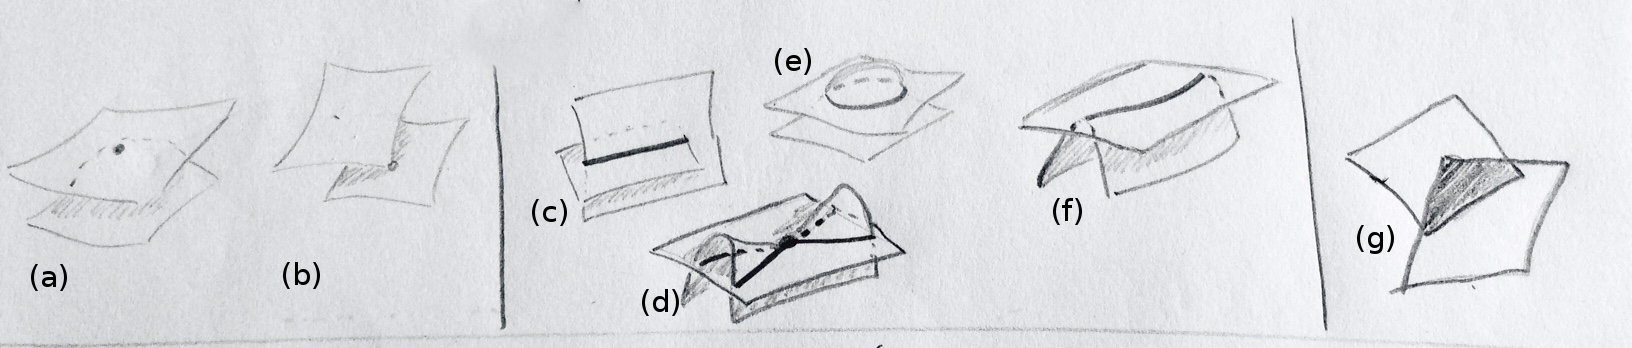
\includegraphics[width=0.95\textwidth]{cas_intersections_carreaux}
	\caption{Configurations possibles pour l'intersection de deux carreaux (non exhaustif).}
	\label{fig:config_intersection_carreaux}
\end{figure}


État de l'art des méthodes pour calculer l'intersection de carreaux paramétriques :
\begin{enumerate}
%	\item Analytiques : limité aux surfaces de degré algébrique très bas (\eg quadriques)
%	\item (Implicitisation (approchée) : )
	\item \anglais{Lattice}.\\
	Les méthodes de ce type consistent à calculer les intersections entre un réseau de \textit{courbes} iso-paramétriques d'un carreau et la \textit{surface} de l'autre carreau \cite{rossignac1987}. 
	Les points d'intersection obtenus sont ensuite connectés pour former les différentes courbes d'intersection. 
	Cette approche, qui présente l'avantage de réduire la complexité du problème, nécessite toutefois de choisir une résolution suffisamment fine pour le réseau des courbes iso-paramétriques afin de capturer correctement la topologie l'intersection. 
	En effet, si cette résolution est trop grossière, la méthode peut échouer à détecter certains détails tels que des points de contact isolés ou des petites boucles, qui apparaissent lorsque les carreaux s'intersectent de façon tangentielle ou quasi-tangentielle.
	
	\item Subdivision.\\
	Le principe de cette approche est de subdiviser de manière récursive le problème d'intersection original en plusieurs sous-problèmes --- typiquement des intersections de régions planes (\eg triangles) --- pour chacun desquels on peut aisément trouver la solution \cite{houghton1985}. 
	Ce type de méthodes produit ainsi un ensemble de segments de la courbe d'intersection, qui doivent également être connectés pour en former les branches. 
	Si la position des points d'intersection ainsi calculés peut être corrigée a posteriori afin de les ramener sur la véritable intersection des carreaux, les approximations utilisées ne garantissent pas la restitution exacte de la topologie de la courbe d'intersection, en particulier dans des cas d'intersections tangentielles ou quasi-tangentielles (illustration faux positif/faux négatif).
	Par ailleurs, le niveau élevé de précision requis par la plupart des applications en CAO nécessite un nombre de subdivisions souvent prohibitif, ce qui disqualifie les méthodes reposant uniquement sur la subdivision.
	%Toutefois, la combinaison de techniques de subdivision adaptative à d'autres méthodes locales de haute précision --- comme les méthodes dites de \textit{suivi} --- permet de concevoir des algorithmes de calcul d'intersection plus efficaces.
	%Les techniques de subdivision adaptative peuvent toutefois être utilisées 

	\item Suivi (\anglais{Marching}).\\
	Les méthodes dites de suivi cherchent dans un premier temps à trouver un point sur chaque branche de la courbe d'intersection. 
	Ensuite, elles procèdent au tracé de ces branches en marchant dans une direction indiquée par la géométrie différentielle locale de la courbe. 
	Afin d'identifier toutes les composantes connexes de la courbe d'intersection, il suffit de trouver les points où les branches ouvertes rencontrent le bord d'un des carreaux, ainsi que les paires de points critiques où les carreaux ont des directions normales parallèles.
	En effet, à chaque branche fermée de la courbe d'intersection est associée une telle paire de points \cite{sederberg1989}.
	En outre, tous les points singuliers de la courbe d'intersection (points de contact isolés, points \guillemets{doubles}, points de branchement) sont également des points critiques.
	\begin{itemize}
		\item trouver toutes les branches, sans doublons
		\begin{itemize}
			\item bords, points critiques
		\end{itemize}
		\item tracer (problème de Cauchy) avec un pas adéquat pour éviter saut/\anglais{jumping}, (\anglais{looping}) et marche-arrière /\anglais{backtracking} et s'arrêter au bon endroit
	\end{itemize}
\end{enumerate}
%pas de paramétrisation explicite (définition procédurale), méthode de Hohmeyer revisitée
%
%\begin{enumerate}
%	\item Subdivision : découper chaque surface en surfaces plus simple (\eg triangles) 
%	\item 
%\end{enumerate}

\par\bigskip

\begin{definition}
	Deux points $\p_1$ et $\p_2$ reposant respectivement sur les carreaux $\Sigma_1$ et $\Sigma_2$ forment une paire de \emph{points critiques} si, pour $i = 1,2$,
	\begin{equation}
		\crossprod{ \unv_{\Sigma_i}\!(\p_i) }{(\p_1 - \p_2)} = \vit{0}.
	\end{equation}
	(Ce sont en effet des points critiques (au sens où le gradient s'y annule) pour la fonction $(\p_1, \p_2) \mapsto \normtwo{\p_1 - \p_2}^2$.)
\end{definition}
\cite{yamaguchi1998} caractérise ces points (avec une autre fonction distance) et donne un algorithme pour tous les trouver




\subsection{Présentation/Vue d'ensemble/Caractéristiques de la méthode retenue}
Adaptation de la méthode préentée dans \cite{hohmeyer1992}, qui est centrée autour du théorème suivant

\begin{theoreme}[Hohmeyer]
	\label{theo:detection_boucles_hohmeyer}
	Soient $\Sigma_1$ et $\Sigma_2$ deux carreaux de continuité $\contdiff{1}$ dont les directions normales sont respectivement contenues dans les ensembles $\mathcal{N}_1$ et $\mathcal{N}_2$. \\
	S'il existe deux vecteurs $\vrm{p}_1$ et $\vrm{p}_2$ tels que, 
	pour tout $\unv_1 \in \mathcal{N}_1$ et pour tout $\unv_2 \in \mathcal{N}_2$,
	\begin{align}
		\dotprod{ \vrm{p}_1 }{ \unv_1 } > 0 &\text{\quad et\quad} \dotprod{ \vrm{p}_1 }{ \unv_2 } < 0, \label{eq:hohmeyer_separation}\\
		\dotprod{ \vrm{p}_2 }{ \unv_1 } > 0 &\text{\quad et\quad} \dotprod{ \vrm{p}_2 }{ \unv_2 } > 0, \label{eq:hohmeyer_hemisphere}
	\end{align}
	alors $\Sigma_1 \cap \Sigma_2$ n'est composée que de 
	\begin{itemize}
		\item points isolés situés sur le bord des carreaux ;
		\item segments ouverts qui ne contiennent ni point double ni point de branchement.
	\end{itemize}
	En outre, la direction tangente $\bt$ d'un tel segment vérifie en tout point
	\begin{equation}
		\dotprod{ \bt }{ (\crossprod{ \vrm{p}_1 }{ \vrm{p}_2 }) } > 0. \label{eq:hohmeyer_monotone}
	\end{equation}
\end{theoreme}


\begin{proof}
	\cf \cite[Théorème~4]{hohmeyer1992}
\end{proof}


Géométriquement, ce théorème peut s'interpréter de la manière suivante. 
D'une part, l'\autoref{eq:hohmeyer_separation} stipule que les ensembles $\mathcal{N}_1$ et $\mathcal{N}_2$ sont strictement séparables par un plan (passant par l'origine et orthogonal à $\vrm{p}_1$). 
D'autre part, l'\autoref{eq:hohmeyer_hemisphere} indique que $\mathcal{N}_1$ et $\mathcal{N}_2$ sont strictement contenus dans un même hémisphère (centré sur l'origine et centré autour du pôle $\vrm{p}_2$). 
Le \autoref{theo:detection_boucles_hohmeyer} donne ainsi une condition suffisante pour garantir que deux carreaux ne s'intersectent pas en une boucle fermée. 
Dans cette situation tous les points nécessaires à la détection de tous les éléments d'intersection (non singuliers) peuvent être trouvés en intersectant les bords de chaque carreau avec la surface de l'autre. 
De plus, l'\autoref{eq:hohmeyer_monotone} simplifie et garantit la validité du tracé des segments d'intersection. [\ldots]
%En effet, comme décrit dans \cite[Section~3.4]{hohmeyer1992}, le produit scalaire $\dotprod{ \bx }{ (\crossprod{ \vrm{p}_1 }{ \vrm{p}_2 }) }$ 
%%\begin{equation}
%%	w := \dotprod{\bx}{\vrm{p}},
%%\end{equation}
%évolue de façon monotone le long du segment, ce qui permet d'éviter le phénomène de marche-arrière lorsqu'il est choisit comme paramètre.



\begin{enumerate}
	\item Détection des branches (composantes connexes) de la courbe d'intersection
	\begin{enumerate}
		\item Subdivision récursive des carreaux en régions qui
		\begin{itemize}
			\item sont clairement disjointes (test de séparation de volumes englobants \cite{eberly1999})
			\item ou bien s'intersectent de façon tangentielle
			\item ou bien ne peuvent pas s'intersecter en une boucle (critère d'élimination des boucles basé sur les enveloppes des normales basé sur le \autoref{theo:detection_boucles_hohmeyer})
		\end{itemize}
		\item Intersection entre les bords d'une région et la surface de l'autre, et vice versa (intersection arc-carreau)
		\item Subdivision récursive en régions qui
		\begin{itemize}
			\item sont clairement disjointes
			\item ne s'intersectent qu'en un seul segment transverse (pas de singularité), que l'on peut tracer sans ambiguïté (pas de saut d'une branche à l'autre)
		\end{itemize}
	\end{enumerate}
	

	\item Représentation des courbes d'intersection
	\begin{enumerate}
		\item le degré algébrique ainsi que le genre topologique des courbes solutions du système \eqref{eq:intersection_2_carreaux} augmentent tellement vite avec le degré des polynômes $\bs^i$ qu'il n'est pas envisageable de les représenter par des arcs paramétriques polynomiaux (\eg la courbe d'intersection de deux carreaux bi-cubiques est de degré 324 et de genre topologique 433 \cite{katz1988}).
		\item on a tout de même besoin d'un type de représentation permettant une évaluation précise des courbes d'intersection
		\item (compte tenu du niveau de précision exigé, une approximation paramétrique polynomiale globale ou \piecewise\ (spline) nécessiterait un volume excessif de données)
		\item on choisit donc d'adopter une représentation \textit{procédurale}
		\begin{enumerate}
			\item approximation linéaire par morceaux (polyligne) $(x,y,z,u_1,v_1,u_2,v_2)$
			\item on peut évaluer précisément n'importe quel point sur la courbe en évaluant d'abord la polyligne puis en raffinant le résultat de façon itérative (projection sur la véritable intersection)
			\item[$\Rightarrow$] un faible volume de données est stocké mais permet d'évaluer la courbe avec une précision arbitraire
		\end{enumerate}
	\end{enumerate}
	
	
	\item Tracé des courbes d'intersection
	\begin{enumerate}
		\item le critère d'élimination des boucles assure la monotonie de la paramétrisation de chaque segment d'intersection (pas de marche-arrière)
		\item problème aux limites (on connaît les deux extrémités du segment avant même de tracer la courbe) au lieu de problème de Cauchy (de valeurs initiales)
	\end{enumerate}
\end{enumerate}


\par\bigskip

Apports/modifications
\begin{enumerate}
	\item représentation des polynômes dans les bases de Bernstein \textit{et} Chebyshev (pour les arcs et carreaux) $\to$ on tire parti des avantages de chaque base pour les différentes étapes de l'algorithme :
	\begin{itemize}
		\item base de Bernstein (Bézier) 
		\begin{itemize}
			\item[+] propriété d'enveloppe convexe $\to$ tests de séparation
			\item[$\Rightarrow$] utilisée pour décrire localement les régions de carreau/arc
		\end{itemize}
		\item base de Chebyshev
		\begin{itemize}
			\item[+] évaluation efficace (Clenshaw) $\to$ méthodes itératives de type Newton qui nécessitent de nombreuses évaluations
			\begin{itemize}
				\item recherche/raffinement d'un point d'intersection arc-carreau
				\item recherche/raffinement d'une paire de points critiques
				\item raffinement d'un point d'intersection (entre 2 ou 3 carreaux)
			\end{itemize}
			\item[+] orthogonalité $\to$ économisation
			\item[+] FFT $\to$ (calcul du carreau pseudo-normal?)
			\item[$\Rightarrow$] utilisée pour décrire le carreau/arc \guillemets{racine}
		\end{itemize}
		\item changement de base par un produit matrice vecteur, matrice de passage donnée par \cite{rababah2003}
		\item on dérive des techniques pour les deux bases et pour les arcs et carreaux
		\begin{enumerate}
			\item extraction d'un bord de carreau sous la forme d'un arc
			\item subdivision : De Casteljau/\guillemets{Reparamétrisation affine}, généralisation de \cite{fournier1994} (cas particulier degré 3 et subdivision au milieu, \ie $u = v = 0$), à mettre en annexe
			\item boîtes englobantes orientées : heuristiques, \cite{munkberg2010} (Bernstein) et extension de \cite{campagna1997} (Chebyshev), à mettre en annexe et comparer complexité de construction et volume des boîtes)
		\end{enumerate}
	\end{itemize}
\end{enumerate}




\section{Intégration temporelle}
Suivi lagrangien de marqueurs (points de collocation, n\oe uds de la grille CGL)

\subsection{Advection dans champ de vecteur vitesse connu}
\begin{enumerate}
	\item Intégration explicite du vecteur vitesse des marqueurs lagrangiens (typiquement Runge-Kutta à l'ordre 4)
	\item Pas vraiment le cas dans les applications visées, mais on peut imaginer des situations de ce type (\eg déformation d'un solide sous l'effet d'efforts aérodynamiques $\to$ vitesse donnée par des solveurs de mécanique des structures/fluides)
\end{enumerate}



\subsection{Propagation suivant une vitesse normale donnée}
\subsubsection{Discrétisation de l'EdS propre d'un carreau paramétrique}
\label{section:discretisation_EdS_propre_carreau}
Entrée : vecteur position $\bx_{i,j}^{(k)}$ et vitesse normale $\nu_{i,j}^{(k)}$ de chaque marqueur lagrangien au $k$-ième instant, pas de temps $\Delta t$ (\ie $\rho = \nu \Delta t$)
\begin{enumerate}
	\item transformation directe (de l'espace physique vers l'espace spectral) pour construire les polynômes d'interpolation du vecteur position et de la vitesse normale
	\item construction des polynômes dérivés 
	\item transformation inverse pour évaluer les dérivées $\bsu$ et $\bsv$ aux n\oe uds CGL $(u_i,v_j)$
	\item calcul de la normale aux n\oe uds CGL
	\begin{equation}
		\unv = \unitized{\crossprod{\bsu}{\bsv}}
	\end{equation}
	\item calcul de la composante tangentielle du déplacement vers l'EdS propre aux n\oe uds CGL
	\begin{equation}
		\vrm{t} = \frac{
				\left( \nu_v I_{1,2} - \nu_u I_{2,2} \right) \bsu + 
				\left( \nu_u I_{1,2} - \nu_v I_{1,1} \right) \bsv
			}{
				I_{1,1} I_{2,2} - I_{1,2}^2
			}.
	\end{equation}
	\item on pose $\tau = \min\left\{\Delta t, \displaystyle\frac{\lambda}{\displaystyle\max_{i,j} \normtwo{\vrm{t}_{i,j}^{(k)} }} \right\}$ ($\lambda \leq 1$) et on avance dans le temps d'un pas $\tau$\\(ATTENTION : $\tau$ doit être le même pour tous les carreaux!)
	\begin{equation}
		\bx_{i,j}^{(k+1)} = \bx_{i,j}^{(k)} + \tau \nu_{i,j}^{(k)} 
		\left( 
			\tau \vrm{t}_{i,j}^{(k)} + \sqrt{1 - \tau^2 \normtwo{\vrm{t}_{i,j}^{(k)}}^2} \unv_{i,j}^{(k)}
		\right)
	\end{equation}
	
	\item Différence avec le simple transport suivant la normale
	\begin{itemize}
		\item on se bouge suivant la normale à l'EdS propre au lieu de la normale à l'interface
		\[
			\bx^{(k+1)} = \bx^{(k)} + \tau \nu^{(k)} \unv^{(k+1)}
		\]
		au lieu de 
		\[
			\bx^{(k+1)} = \bx^{(k)} + \tau \nu^{(k)} \unv^{(k)}
		\]
		$\sim$ schéma semi-implicite en temps?
		\[
			\sqrt{1 - y} = 1 + \bigO{y},
		\]
		donc
		\[
			\left( \bx^{(k+1)} - \bx^{(k)} \right) - \tau \nu^{(k)} \unv^{(k)} = \tau^2 \nu^{(k)} \vrm{t}^{(k)} + \bigO{\tau^3}
		\]
		et donc la différence est d'ordre 2 en temps
		\item si $\nu$ est uniforme (\ie $\nu_u = \nu_v = 0$) alors construire l'EdS propre revient à propager suivant la normale à l'interface courante. 
		En outre, la direction de $\unv$ reste constante en chaque point. 
		En revanche, le signe de $\unv$ peut s'inverser lorsque $\nu \tau$ dépasse le plus petit rayon de courbure local ($\to$ offset dégénéré \ldots).
	\end{itemize}
\end{enumerate}

\subsubsection{Discrétisation de la pseudo-EdS d'une arête \brep\ convexe}%d'un arc de courbe}
\begin{enumerate}
	\item \cf \autoref{section:parametrisation_pseudo_EdS_arete}
	\item paramétrisation polynomiale
	\begin{enumerate}
		\item[$\Rightarrow$] approximation (remarque sur les paramétrisations rationnelles exactes \cite{peternell1997})
		\item[$\Rightarrow$] degré à choisir
	\end{enumerate}
	\item décrire l'échantillonnage de la courbe d'intersection ($\Right{\bp}$, $\Left{\bp}$ et $\bg$) aux n\oe uds CGL pour le paramètre de Hohmeyer $w = \dotprod{\vrm{p}}{\bg}$
	\begin{enumerate}
		\item méthode procédurale : on s'appuie sur une polyligne et on affine par la méthode de Newton (expliciter l'itération)
		\item calcul de la direction tangente $\vrm{t} = \unitized{\bgw}$ (\cf géométrie différentielle des courbes d'intersection transverses, s'assurer de la positivité du produit scalaire avec le vecteur de paramétrisation de Hohmeyer $\vrm{p}$)
	\end{enumerate}
	\item évaluation des courbes \guillemets{limites} $\Right{\eos}$ et $\Left{\eos}$
	\item échantillonnage des arc caractéristiques aux n\oe uds CGL en $v \in \chebinterval$
	\begin{enumerate}
		\item en pratique, pour garantir la validité des courbes d'intersections tangentielles entre les carreaux de l'EdB, on choisit 
		\[
			\bo_i = \bg_i + \frac{\dotprod{\left( \Right{\eos}_i + \Left{\eos}_i - 2 \bg_i \right)}{\bt_i}}{2}\bt_i,
		\]  
		et, puisque $\lo{v} = -1$ et $\hi{v} = 1$,
		\[
			r_{i,j} = 
			\frac{
				\left(1 - v_j\right) \normtwo{\Right{\eos}_i - \bo_i} + \left(1 + v_j\right) \normtwo{\Left{\eos}_i - \bo_i}
			}{
				2
			},
		\]
		et
		\[
			\br_{i,j} = 
	        \cos\left( \frac{1 + v_j}{2} \theta_i \right) \Right{\br}_i +
	        \sin\left( \frac{1 + v_j}{2} \theta_i \right) \Right{\br}^{\perp}_i,
		\]
		\item[$\Rightarrow$] on a alors 
		\[
			\eos_{i,j} = \bo_{i} + r_{i,j} \br_{i,j}
		\]
	\end{enumerate}
	\item à noter qu'ici on n'utilise ni $\tau$ ni $\nu$
	\item les nouveaux carreaux ainsi créés seront ensuite propagés comme les autres aux instants suivants
\end{enumerate}



\subsubsection{Discrétisation de la pseudo-EdS d'un sommet \brep\ non-concave}
\begin{enumerate}
	\item polygone sphérique découpé en quadrilatères (\cf \autoref{section:quadrangulation_polygone_spherique})
	\begin{itemize}
		\item construction d'un carreau bilinéaire (échantillonnage aux n\oe uds de la grille CGL)
		\item projection sur la sphère
		\item[$-$] spectre de Chebyshev plus étalé (degré plus élevé pour une précision donnée)
	\end{itemize}
	\item ajustement de carreau sphérique à un nuage de points
	\begin{itemize}
		\item échantillonnage aux n\oe uds de la grille CGL du carreau obtenu par la méthode décrite dans la \autoref{section:ajustement_carreau_spherique}
		\item[$+$] spectre de Chebyshev plus compact
	\end{itemize}
\end{enumerate}




\section{Amélioration de la stabilité numérique}
\label{section:instabilités}

\subsection{Réduction de l'erreur d'aliasing}

méthode proposée par \cite{rahimian2015} difficile à appliquer dans notre cas car 
\begin{enumerate}
	\item les carreaux de surface ont un bord, 
	\item l'espacement non-uniforme des marqueurs lagrangiens (images des n\oe uds CGL) impose une forte contrainte CFL sur leurs déplacements
\end{enumerate}

\subsection{Prévention des singularités géométriques}
Notre approche permet naturellement de supporter les singularités géométriques de l'interface, à condition qu'elles soient localisées à l'intersection d'au moins deux carreaux de surface (et donc sur leur bord).
En revanche, les singularités qui se forment au sein d'un même carreau provoquent de sérieux problèmes de stabilité numérique.
On distingue 2 types de singularités (\cite[p.320]{patrikalakis2009}) :
\begin{itemize}
	\item points irréguliers (auto-intersection locale) (normale et plan tangent non définis, $\determinant{\fff} = 0$) $\Rightarrow$ oscillations de Gibbs
	\item auto-intersections globales (non-injectivité de la paramétrisation) : ne pose pas de problème de stabilité numérique mais viole la définition de variété
\end{itemize}

\begin{itemize}
	\item \cite{jiao2001} (en 2D, \ie l'interface est une courbe) : 
	\item \cite{farouki1986} donne les conditions pour qu'une interface (représentée par une mosaïque de carreaux paramétriques) propagée à vitesse normale uniforme devienne localement singulière
\end{itemize}

pistes de résolution envisageables
\begin{enumerate}
	\item approximation non dégénérée \cite{farouki1986}
	\item tracé des courbes iso-courbure critique \cite[chap.8]{patrikalakis2009} pour redéfinir les carreaux de surfaces concernés
	\item redécoupage des carreauxle long des courbes d'auto-intersection \cite{urick2019} 
	\begin{itemize}
		\item élimine les régions problématiques
		\item produit des nouveaux carreaux non-restreints
		\item (assure l'étanchéité de la mosaïque de carreaux)
	\end{itemize}
	
\end{enumerate}

%bilan : pas de solution simple, reste un gros point faible de l'approche choisie\ldots
bilan : en l'état actuel, problème non résolu mais idées solutions prometteuses